\chapter{量子接收机实验平台搭建}
前面两章,我们分别研究了单符号的QAM信号量子接收机,
以及多个符号的编码后二元调制信号量子接收机。
通过理论分析和数值仿真分析,我们证明了
我们提出的量子接收机能够突破经典检测极限——标准量子极限。
然而到目前为止,
从实验上对量子接收机进行论证的工作仅停留在有限的几种方案当中,
对于更多的方案以及他们的工程实现还有待进一步研究。
为了后续的实验研究工作,我们在现阶段进行量子接收机实验平台
搭建工作,希望能够完成一个初步的实验平台。


\section{实验原理及实验平台搭建}
最早对量子接收机进行实验验证的工作要追溯到2006 年 C. W. Lau等人
开始进行二元调制信号的Kennedy接收机和Dolinar接收机的实验验证\cite{lau2006binary},
但是很遗憾受限于实验条件Dolinar接收机没能突破标准量子极限。
当时实验装置采用空间光路,位移操作通过一个空间光马赫曾德干涉仪实现,
由于对幅度调制的精确控制达不到要求,使得Dolinar接收机性能不理想。
到2007年,R. L. Cook终于从实验上验证了Dolinar接收机能够达到Helstrom极限\cite{cook2007optical}。
从这两个实验及后续的一些实验来看\cite{wittmann2008demonstration,wittmann2010demonstration,tsujino2010sub,
tsujino2011quantum,becerra2011m,chen2012optical,muller2012quadrature,becerra2013experimental,
becerra2015photon},
实验上目前实现量子接收机的难点在于
具有光子数分辨能力的高量子效率低暗计数的单光子探测器和对位移操作的精确实现。
对于前者,实验上通过采用死区时间小探测效率在65\%左右的APD单光子探测器实现,
也有实验采用超导TES单光子探测器以达到非常高的量子效率\cite{tsujino2011quantum}。
而具有光子数分辨能力的探测器能够使得接收机鲁棒性更强已被
理论和实验验证\cite{izumi2013quantum,li2013suppressing,becerra2015photon}。
这里我们考虑超导探测器需要很低的温度控制,
对实验环境要求太高,所以我们采用大多数研究组都采用的APD单光子探测器。
我们采购的是EXCELITAS 公司型号为SPCM-AQRH-16单光子探测器,
典型的死区时间为20ns,暗计数只有25cps,在633nm波段探测效率
>65\%。
对于后者,实验上有两种实现方案,一种是利用一个马赫曾德干涉仪,它
通过主动的反馈控制将两个臂的光程差进行锁定,
以保证足够的条纹可见度\cite{becerra2013experimental,
becerra2015photon};另一种方案是利用偏振复用,
其中一个偏振当做信号而另一个偏振分量当做本振,最后通过一个偏振分束器(PBS)进行干涉\cite{wittmann2008demonstration,wittmann2010demonstration},
由于本振和信号通过相同的光路,所以不存在干涉的两个臂的光程差不稳定的问题,
但是这种方案对信道保偏性和调制器的偏振特性要求较高,只适合空间光路。
由于后面一种方案便于在空间光路中实现,
所以我们采用后面这种方案实现精密的位移操作。


\begin{figure}
\centering
  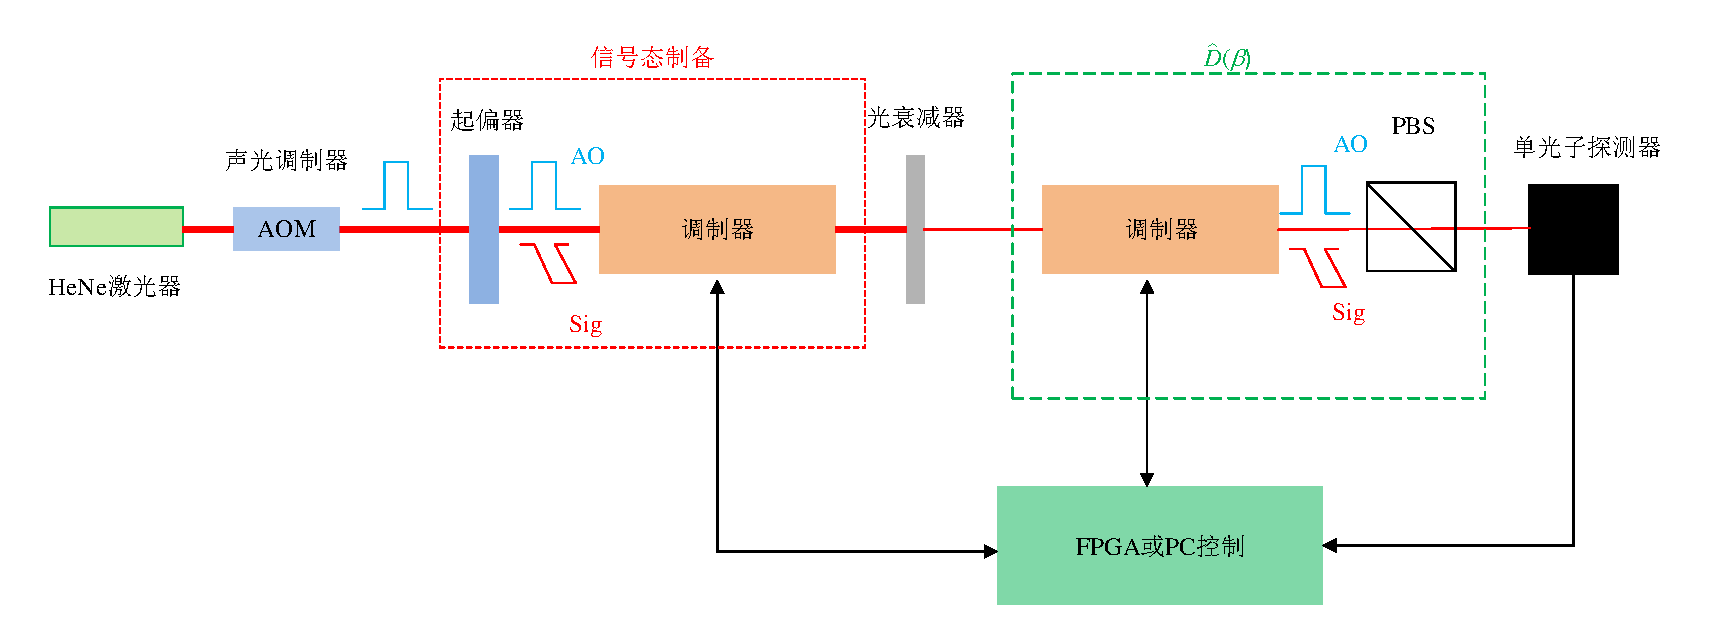
\includegraphics[width=\textwidth]{figures/chap5/experiment-schematic}
  \caption{量子接收机实验原理图}
  \label{fig:experiment-schematic}
\end{figure}



实验原理图如图\ref{fig:experiment-schematic}所示,
HeNe激光器发出的连续光经过声光调制器(AOM)被斩成光脉冲,
然后经过起偏器得到水平偏振分量和垂直偏振分量。
其中水平偏振分量为信号态(Sig),垂直偏振分量为辅助场(AO),在接收端被用作本振场(LO)。
接着,调制器通过基于非线性晶体的电光调制器,
对两个偏振分量进行相移,由于非线性特性导致相移量存在一个差值$\Delta \phi$。
对于BPSK调制,通过控制调制电压使得$\Delta \phi$取$0$和$\pi$,
对于一般的PSK调制只需要控制调制电压就行。
最后信号通过光衰减片模拟的有损信道,
到达接收端,这样就完成了信号态的制备。
用琼斯矩阵表示为
\begin{equation}
\ket{\psi_{Sig, AO}}(\Delta \phi) = \begin{bmatrix}
                            e^{j \Delta \phi}\sqrt{n_{Sig}} \\
                            \sqrt{n_{AO}} 
                        \end{bmatrix}
\end{equation}
在接收端接收机通过一个电光调制器
和一个偏振分束器
实现位移操作,然后进行光子计数。
设调制器导致的相移为$\Delta \phi' + \pi$,
PBS的极化矢量为$\vec{p} = [\sqrt{T} \quad \sqrt{1-T}]$,$T$为透过率,
那么进入单光子计数器钱的光场为
\begin{equation}
\bra{\vec{p}} \ket{\psi_{Sig, AO}}(\Delta \phi + \Delta \phi') \\
             =  \sqrt{T}\sqrt{n_{Sig}} - \sqrt{1-T}\sqrt{n_{AO}} e^{j(\Delta \phi + \Delta \phi')} 
\end{equation}
若PSB与信号偏振态的夹角$\theta$非常小,
那么透过率$T = \cos^2 \theta \approx 1$,
那么上述相当于完成位移操作
\begin{equation}
\hat{D}(\beta) = \hat{D}(\sqrt{n_{AO}}\sqrt{1-T} e^{j \Delta\phi'}).
\end{equation}
特别的,当$T = \frac{n_{AO}}{n_{Sig} + n_{AO}}$时,
到达探测的脉冲中的平均光子数为
\begin{equation}
\bar{n} = \frac{n_{Sig} n_{AO}}{n_{Sig} + n_{AO}} \left|1 - e^{j\Delta \phi + j \Delta \phi'} \right|^2.
\end{equation}
当且仅当$\Delta \phi + \Delta \phi'$ 是$2\pi$的整数倍时,
恰好光强为0,此时位移操作恰好把信号场归零。

\section{Kennedy接收机实验}

在实验的初期,我们对最简单的Kennedy接收机进行实验验证。
对于Kennedy接收机,我们可以简化实验结构。
在接收端由于采用的是恒定的位移场,所以接收端不需要电光调制器。
在发送端,由于只需要产生$0$和$\pi$相位的相移量,
所以可以用一个半波片替代调制器。




\begin{figure}
\centering
  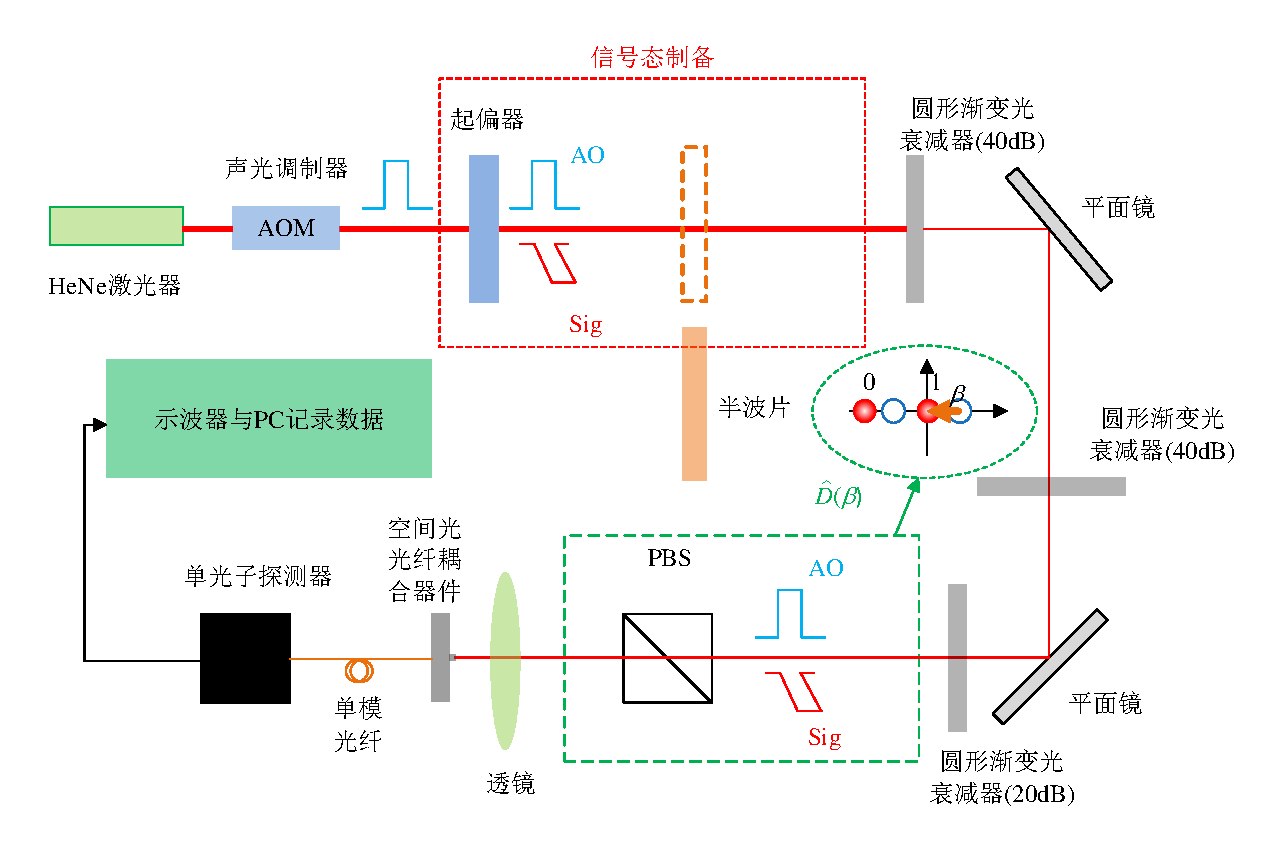
\includegraphics[width=\textwidth]{figures/chap5/Kennedy-receiver-diagram}
  \caption{Kennedy接收机实验光路示意图}
  \label{fig:Kennedy-receiver-diagram}
\end{figure}

实验光路示意图如图\ref{fig:Kennedy-receiver-diagram}所示,
实验照片如图\ref{fig:experiment-photo}所示。
线偏振的信号光通过一个半波片进行调制,
激光器采用JSDU公司生产的型号为1508P-2的氦氖激光器,
它输出0.5mW的532.8nm的线偏光,偏振度高达500:1。 
如果没有半波片意味着相移为$0$,
对应于符号$\ket{\alpha}$;
如果发送光路插入了半波片意味着相移为$\pi$,
对应于符号$\ket{-\alpha}$。
而在接收端,没有加半波片,
意味着位移操作为$\hat{D}(-\alpha)$。
实验光路取夹角为$45 \deg$,因此系统效率最高为50\%。
通过采用一个偏振度高达1000:1的偏振分束器,
可以使得接收端最大光强与最小光强之比达到1:0.55\%,对应的条纹可见度为98.9\% 。
三个圆形渐变衰减片提供最大到100dB的衰减量,
以保证每个光脉冲中平均光子数到单光子量级。
实验中取每个光脉冲宽度为5us,每次试验对符号$\ket{\alpha}$
和$\ket{-\alpha}$各重复$2\times 10^4$次。
在实验过程中,可以通过调节其中一个最大衰减系数为20dB的衰减片,
得到不同光强下的信号,
从而得到不同平均光子数下的平均错误概率。
最后进行光强探测的是Excelitas公司生产的型号为SPCM-AQRH16的单光子探测器。
该探测器探测效率为65\%,初步实验中没有计入该探测效率和耦合损耗的影响。
该探测器暗计数标称为25cps,实验当中由于环境杂散光等原因使得实际暗计数比该数值要大。
实测的暗计数为35.9cps,因此一个光脉冲内的暗计数为$1.795\times 10^{-4}$个。
系统由于采用空间光路耦合,因此对环境光干扰很敏感,实验中通过将接收端
放入一个只有一个开孔的黑色纸盒中,以减少环境光干扰和激光器的散射光干扰。
这个技巧可以将环境光干扰降低至少10dB。


\begin{figure}
\centering
  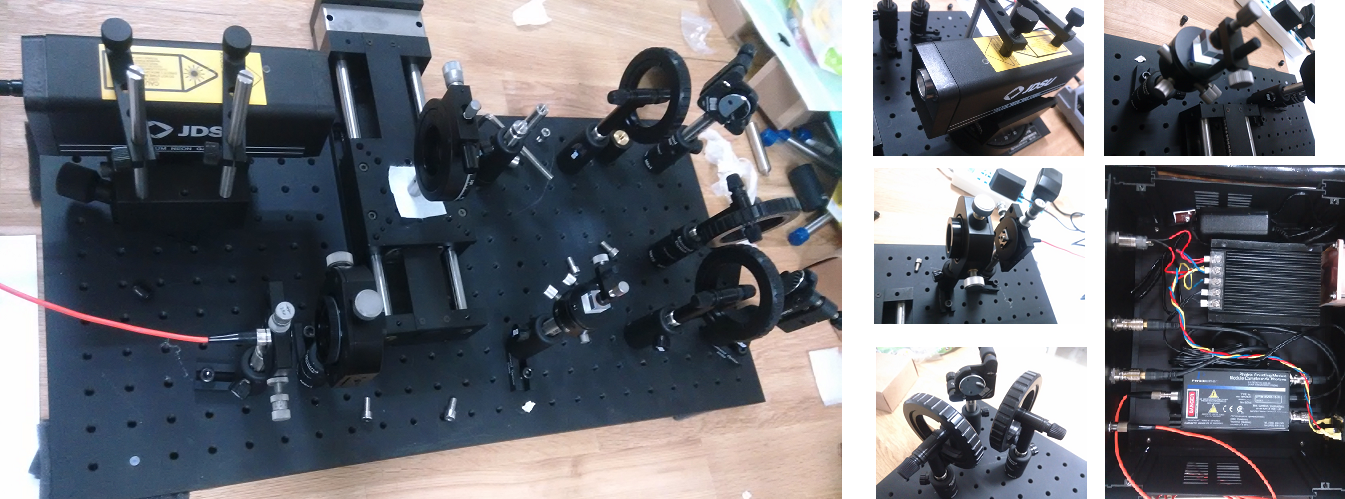
\includegraphics[width=\textwidth]{figures/chap5/experiment-photo}
  \caption{Kennedy接收机实验照片}
  \label{fig:experiment-photo}
\end{figure}


通过改变可变衰减片,
可以制备不同光强下的相干光脉冲。
实验结果如图\ref{fig:kennedy-experiment-error}所示,
其中实验结果用方块表示出来,可以看到,
实验中的Kennedy接收机虽然没能突破效率为1的标准量子极限(SQL),
但是突破了效率为50\%的标准量子极限,最大的收益达到1dB。




\begin{figure}
\centering
  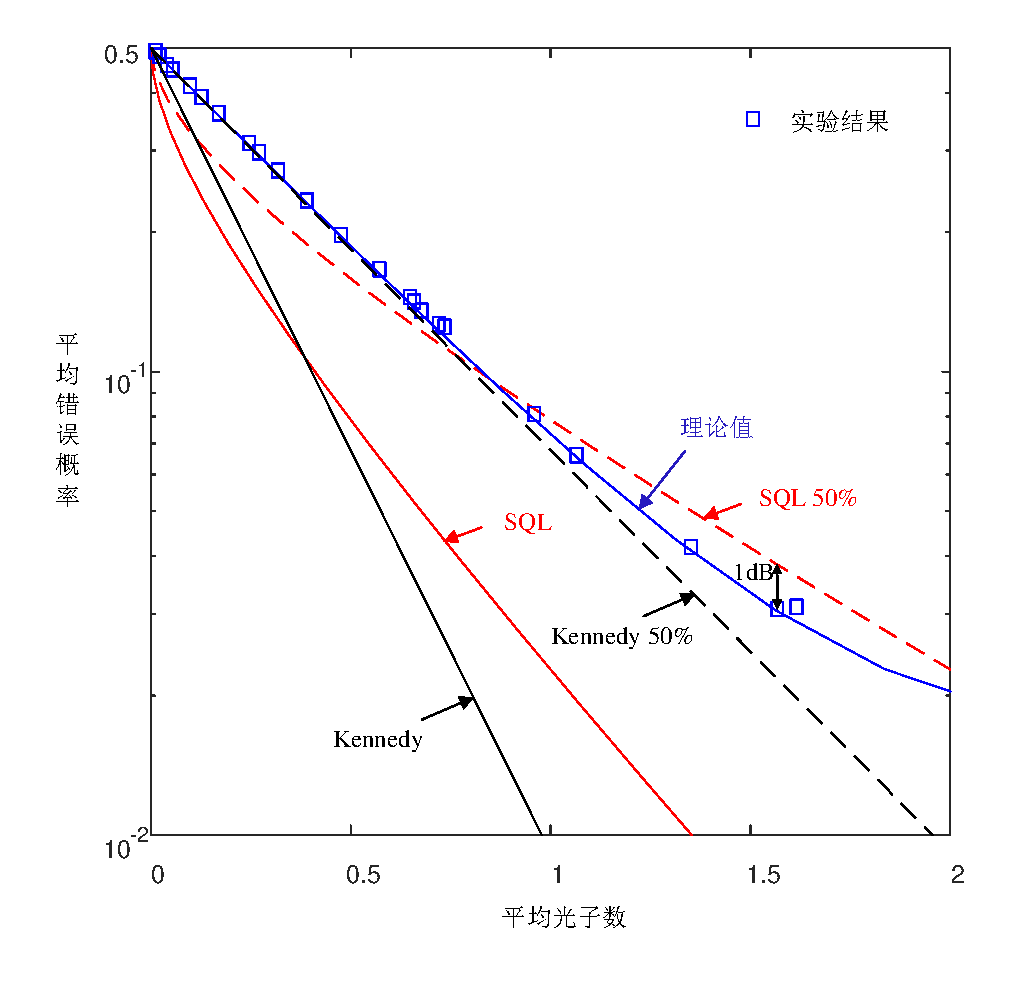
\includegraphics[width=0.6\textwidth]{figures/chap5/kennedy-experiment-error}
  \caption{Kennedy接收机实验结果}
  \label{fig:kennedy-experiment-error}
\end{figure}

